% !TEX TS-program = pdflatex
% !TEX encoding = UTF-8 Unicode

% This is a simple template for a LaTeX document using the "article" class.
% See "book", "report", "letter" for other types of document.

\documentclass[11pt]{article} % use larger type; default would be 10pt

\usepackage[utf8]{inputenc} % set input encoding (not needed with XeLaTeX)

%%% Examples of Article customizations
% These packages are optional, depending whether you want the features they provide.
% See the LaTeX Companion or other references for full information.

%%% PAGE DIMENSIONS
\usepackage{geometry} % to change the page dimensions
\geometry{a4paper} % or letterpaper (US) or a5paper or....
\geometry{margin=.5in} % for example, change the margins to 2 inches all round
% \geometry{landscape} % set up the page for landscape
%   read geometry.pdf for detailed page layout information

\usepackage{graphicx} % support the \includegraphics command and options

% \usepackage[parfill]{parskip} % Activate to begin paragraphs with an empty line rather than an indent

%%% PACKAGES
\usepackage{booktabs} % for much better looking tables
\usepackage{array} % for better arrays (eg matrices) in maths
\usepackage{paralist} % very flexible & customisable lists (eg. enumerate/itemize, etc.)
\usepackage{verbatim} % adds environment for commenting out blocks of text & for better verbatim
\usepackage{subfig} % make it possible to include more than one captioned figure/table in a single float
% package for algorithms
%\usepackage{algorithm} 
%\usepackage{algorithmic}

%%% HEADERS & FOOTERS
\usepackage{fancyhdr} % This should be set AFTER setting up the page geometry
\pagestyle{fancy} % options: empty , plain , fancy
\renewcommand{\headrulewidth}{0pt} % customise the layout...
\lhead{}\chead{}\rhead{}
\lfoot{}\cfoot{\thepage}\rfoot{}

%%% SECTION TITLE APPEARANCE
\usepackage{sectsty}
\allsectionsfont{\sffamily\mdseries\upshape} % (See the fntguide.pdf for font help)
% (This matches ConTeXt defaults)

%%% ToC (table of contents) APPEARANCE
\usepackage[nottoc,notlof,notlot]{tocbibind} % Put the bibliography in the ToC
\usepackage[titles,subfigure]{tocloft} % Alter the style of the Table of Contents
\renewcommand{\cftsecfont}{\rmfamily\mdseries\upshape}
\renewcommand{\cftsecpagefont}{\rmfamily\mdseries\upshape} % No bold!
%\renewcommand{\thesection}{\alph{section}}

%%% Import math libraries 
\usepackage{amsmath}
\usepackage{amsfonts}
\newcommand{\norm}[1]{\left\lVert#1\right\rVert}

%%% Import libraries for inserting code 
\usepackage{listings}
\usepackage{color}

\definecolor{dkgreen}{rgb}{0,0.6,0}
\definecolor{gray}{rgb}{0.5,0.5,0.5}
\definecolor{mauve}{rgb}{0.58,0,0.82}

\lstset{frame=tb,
  language=Python,
  aboveskip=3mm,
  belowskip=3mm,
  showstringspaces=false,
  columns=flexible,
  basicstyle={\small\ttfamily},
  numbers=none,
  numberstyle=\tiny\color{gray},
  keywordstyle=\color{blue},
  commentstyle=\color{dkgreen},
  stringstyle=\color{mauve},
  breaklines=true,
  breakatwhitespace=true,
  tabsize=3
}
% use \begin{lstlisting} CODE \end{lstlisting}

%%% syntax for importing figures: 
%\begin{figure}[h!]
%\centering
%\includegraphics[scale=1.0]{path}
%\end{figure} 

%%% END Article customizations

%%% The "real" document content comes below...

\title{Algorithm for batch Bayesian optimization}
\author{}
\date{} % Activate to display a given date or no date (if empty),
         % otherwise the current date is printed 

\begin{document}
%\maketitle

\section*{Batch Bayesian optimization example}

As an example, consider the following function to optimize, 

\begin{equation}
f(x, y) = 1 - (u^2 + v^2 - 0.3 \mathrm{cos} (3 \pi u) - 0.3 \mathrm{cos} (3 \pi v)) \quad u = 1.6 x - .5 \quad v = 1.6 y - .5 
\label{cosines}
\end{equation}

\begin{figure}[h!]
\centering
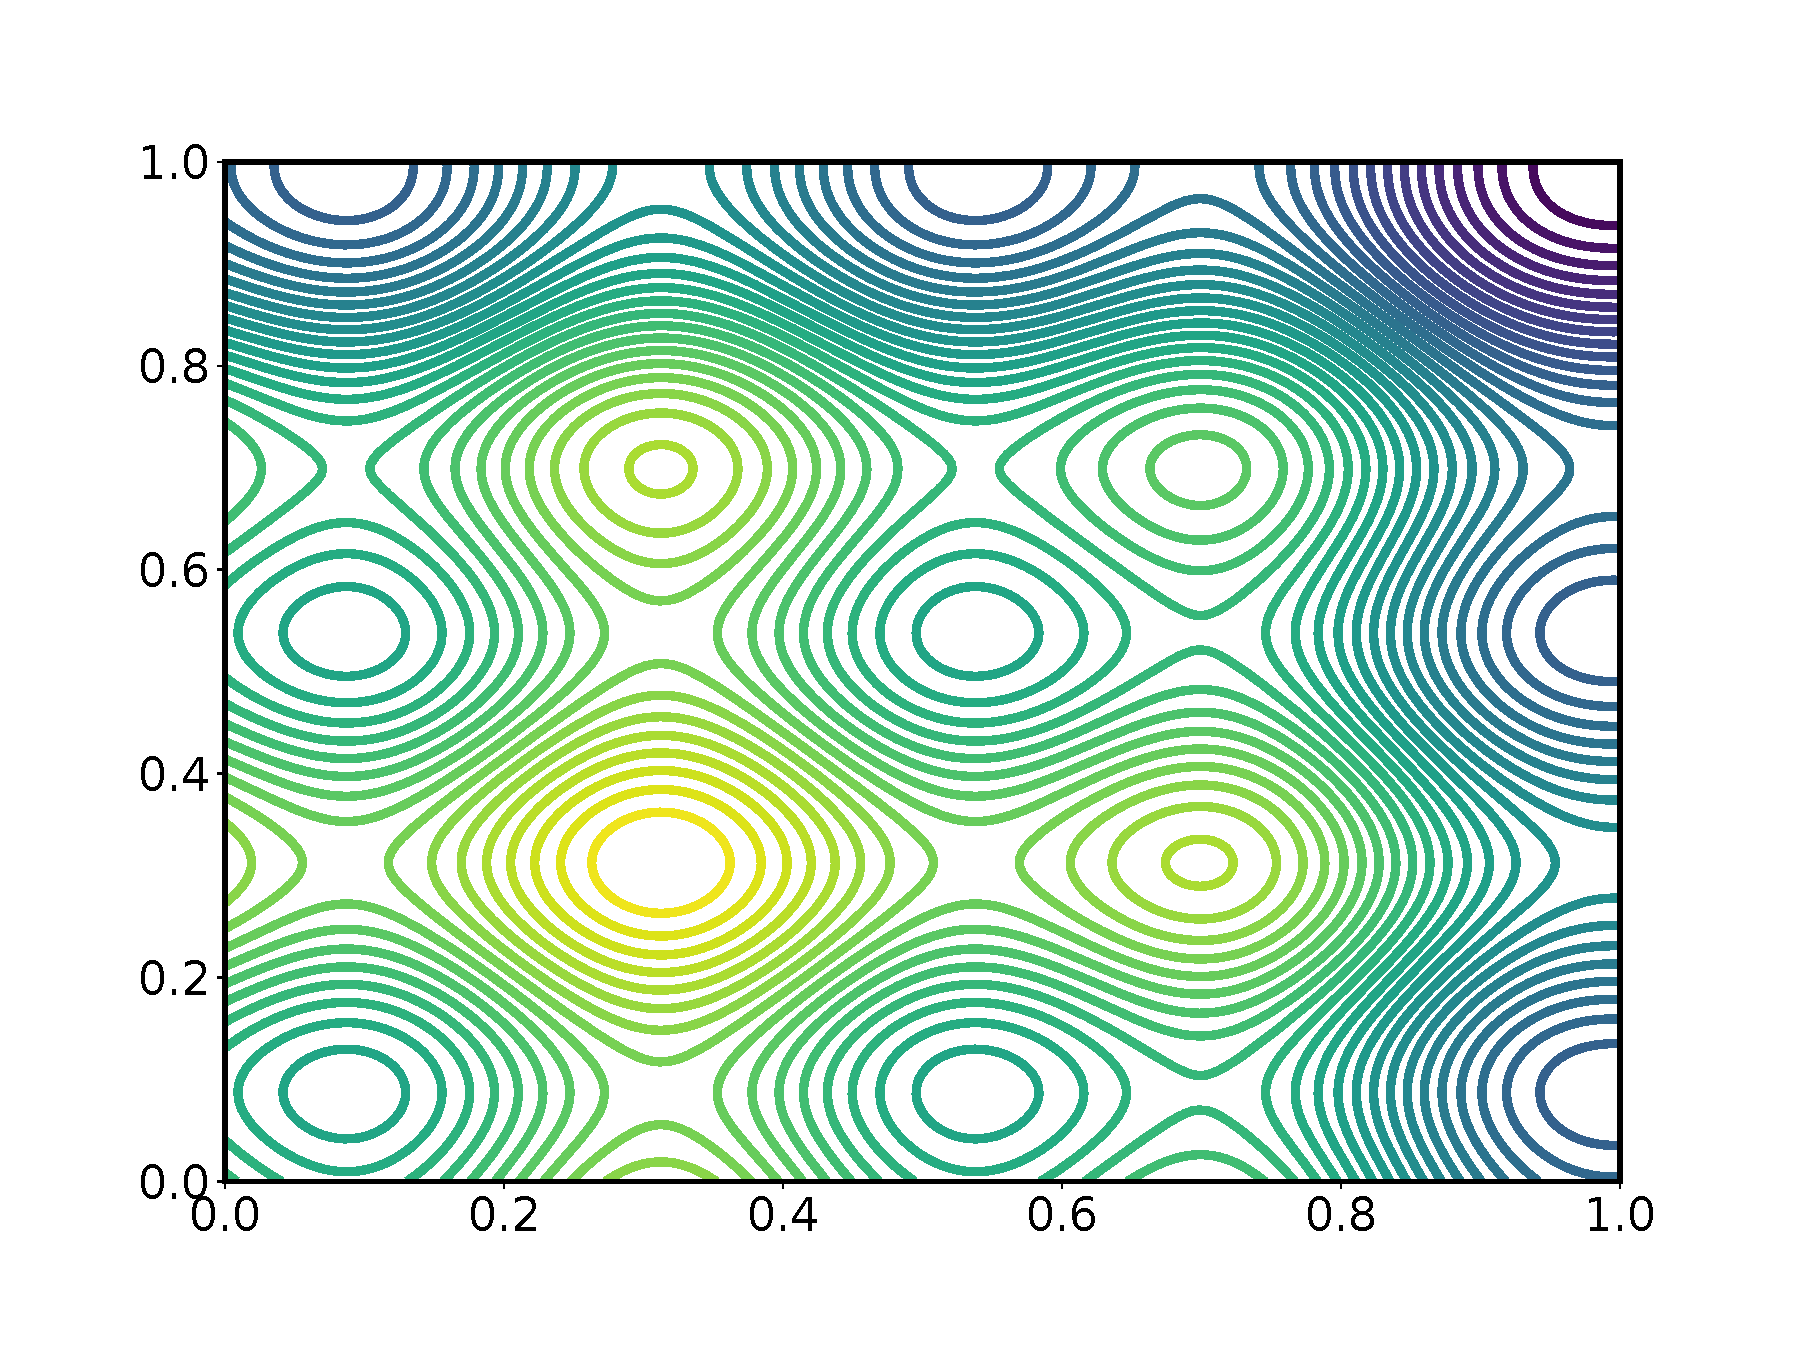
\includegraphics[width=5.in]{Figures/objective.pdf}
\end{figure} 

~\newline
An initial set of 15 points was randomly selected in $[0, 1]^2$ and used to train a neural network to predict the objective. Training data are shown as blue dots and model suggestions for the next experiment are shown as ten orange dots. The regret is the difference between the best possible objective value subtracted by the best value found in the proposed data.  

\begin{figure}[h!]
\centering
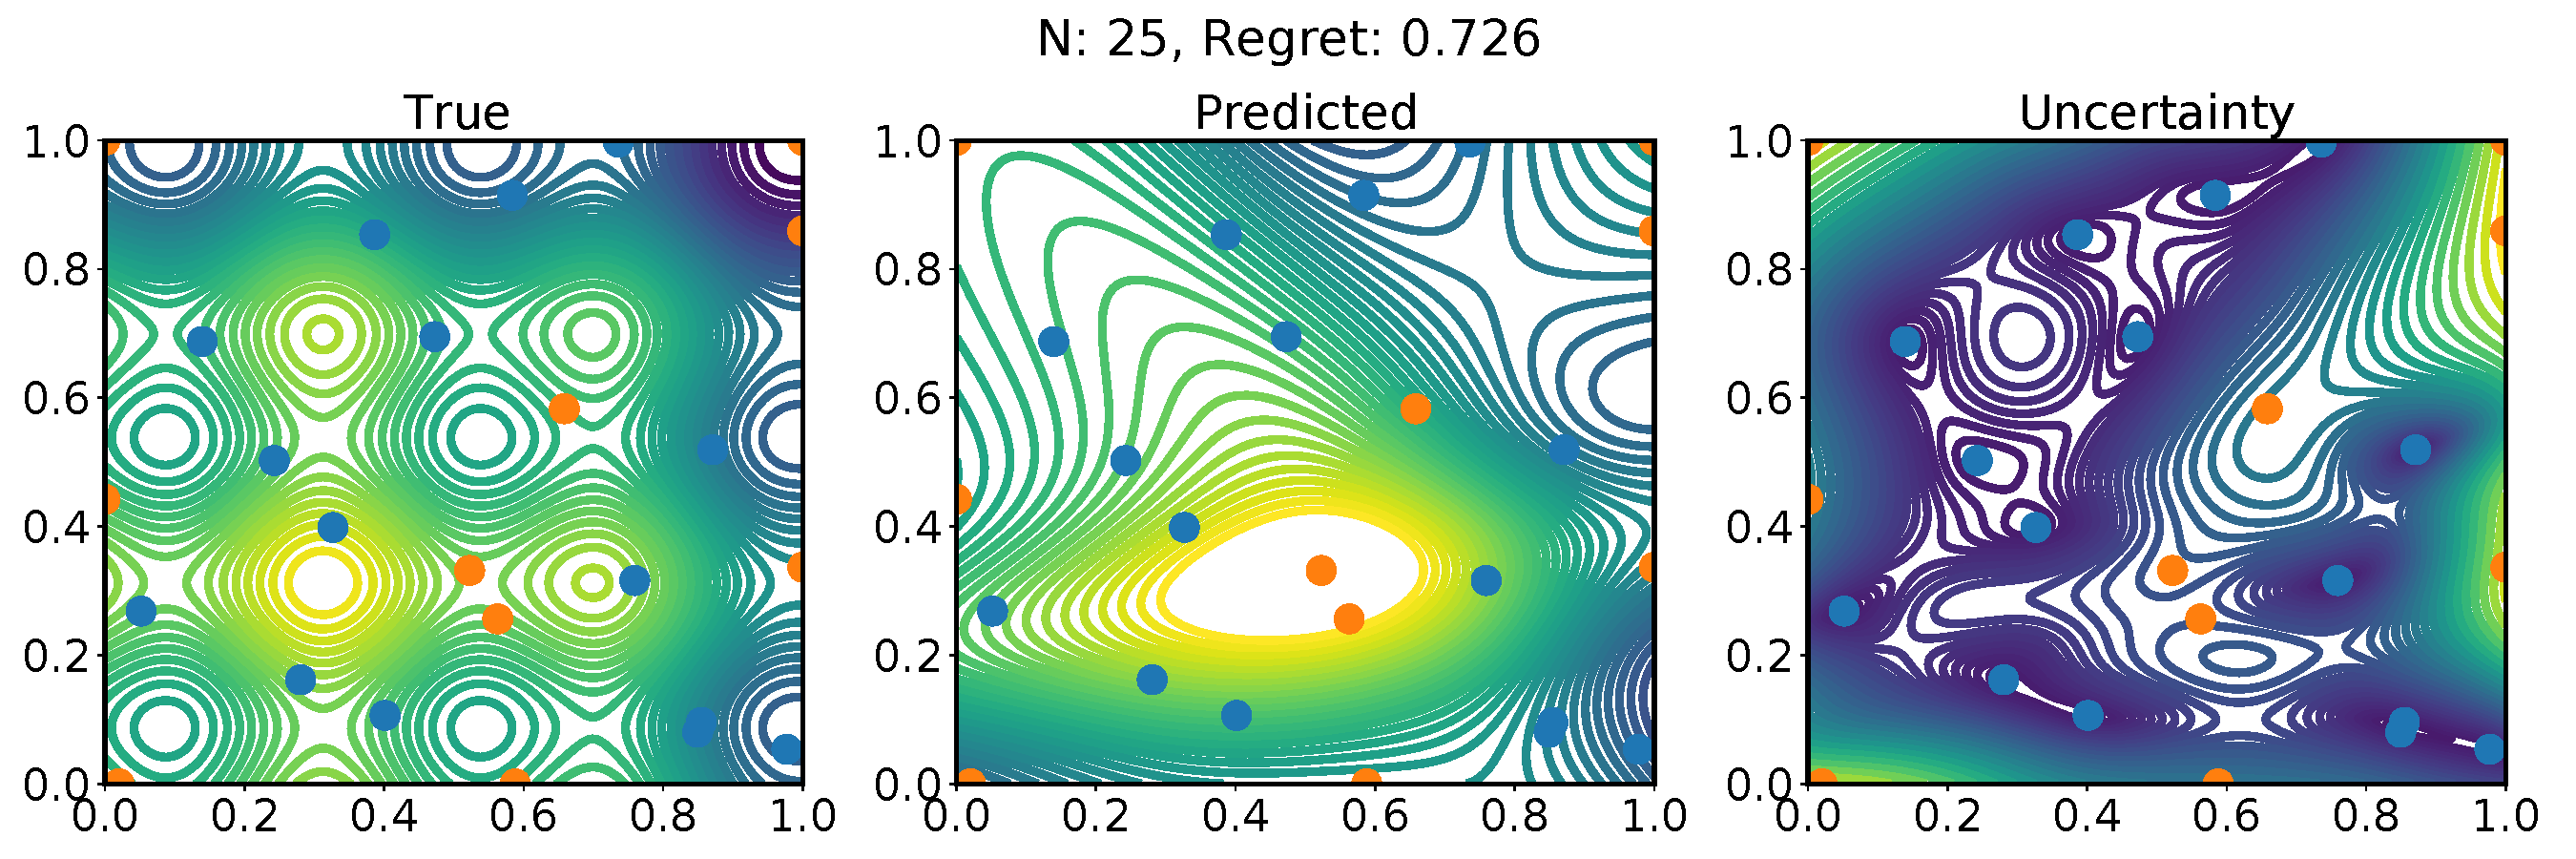
\includegraphics[width=7.5in]{Figures/Cosines_DTL_0.pdf}
\end{figure} 
~\newline
The proposed experimental design includes 10 conditions (orange dots) that exploit and explore the design space. In this initial design, there are several orange dots that occupy the edges/corners of the design space (exploration) and a few orange dots that were sampled where the model predicted higher values for the objective function (exploitation).    

\clearpage
~\newline
All of the orange dots and previously used blue dots were used to assemble a new training set that was used to re-fit the model. In next experimental design, a new set of ten orange dots was proposed. Now that the model is more confident about the edges of the design space, the next experimental design includes many more orange dots in areas where the model expects higher values for the objective function. 

\begin{figure}[h!]
\centering
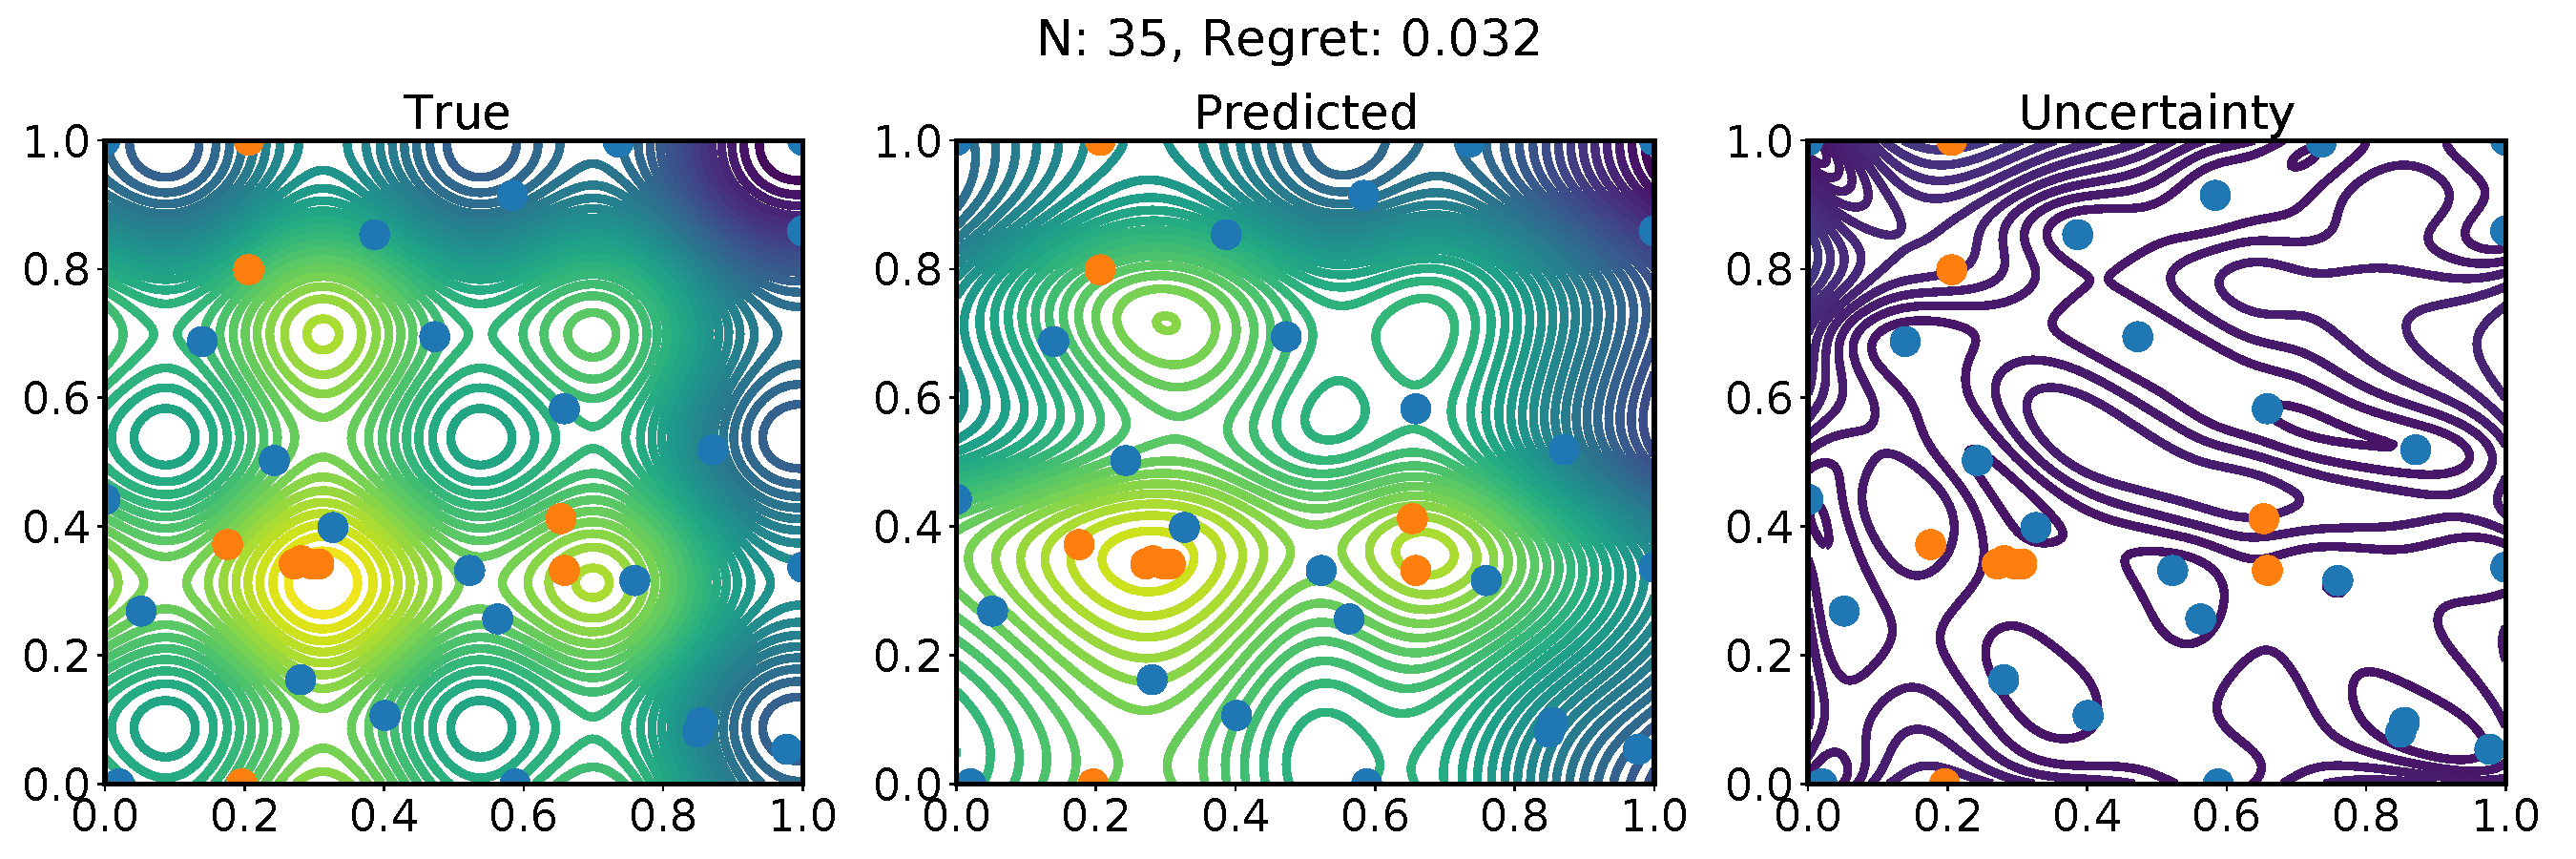
\includegraphics[width=7.5in]{Figures/Cosines_DTL_1.pdf}
\end{figure} 

~\newline 
Once updated with data from the second experimental design, the model is now very confident in the location of the maximum value of the objective function so the final design does not explore beyond that point. 

\begin{figure}[h!]
\centering
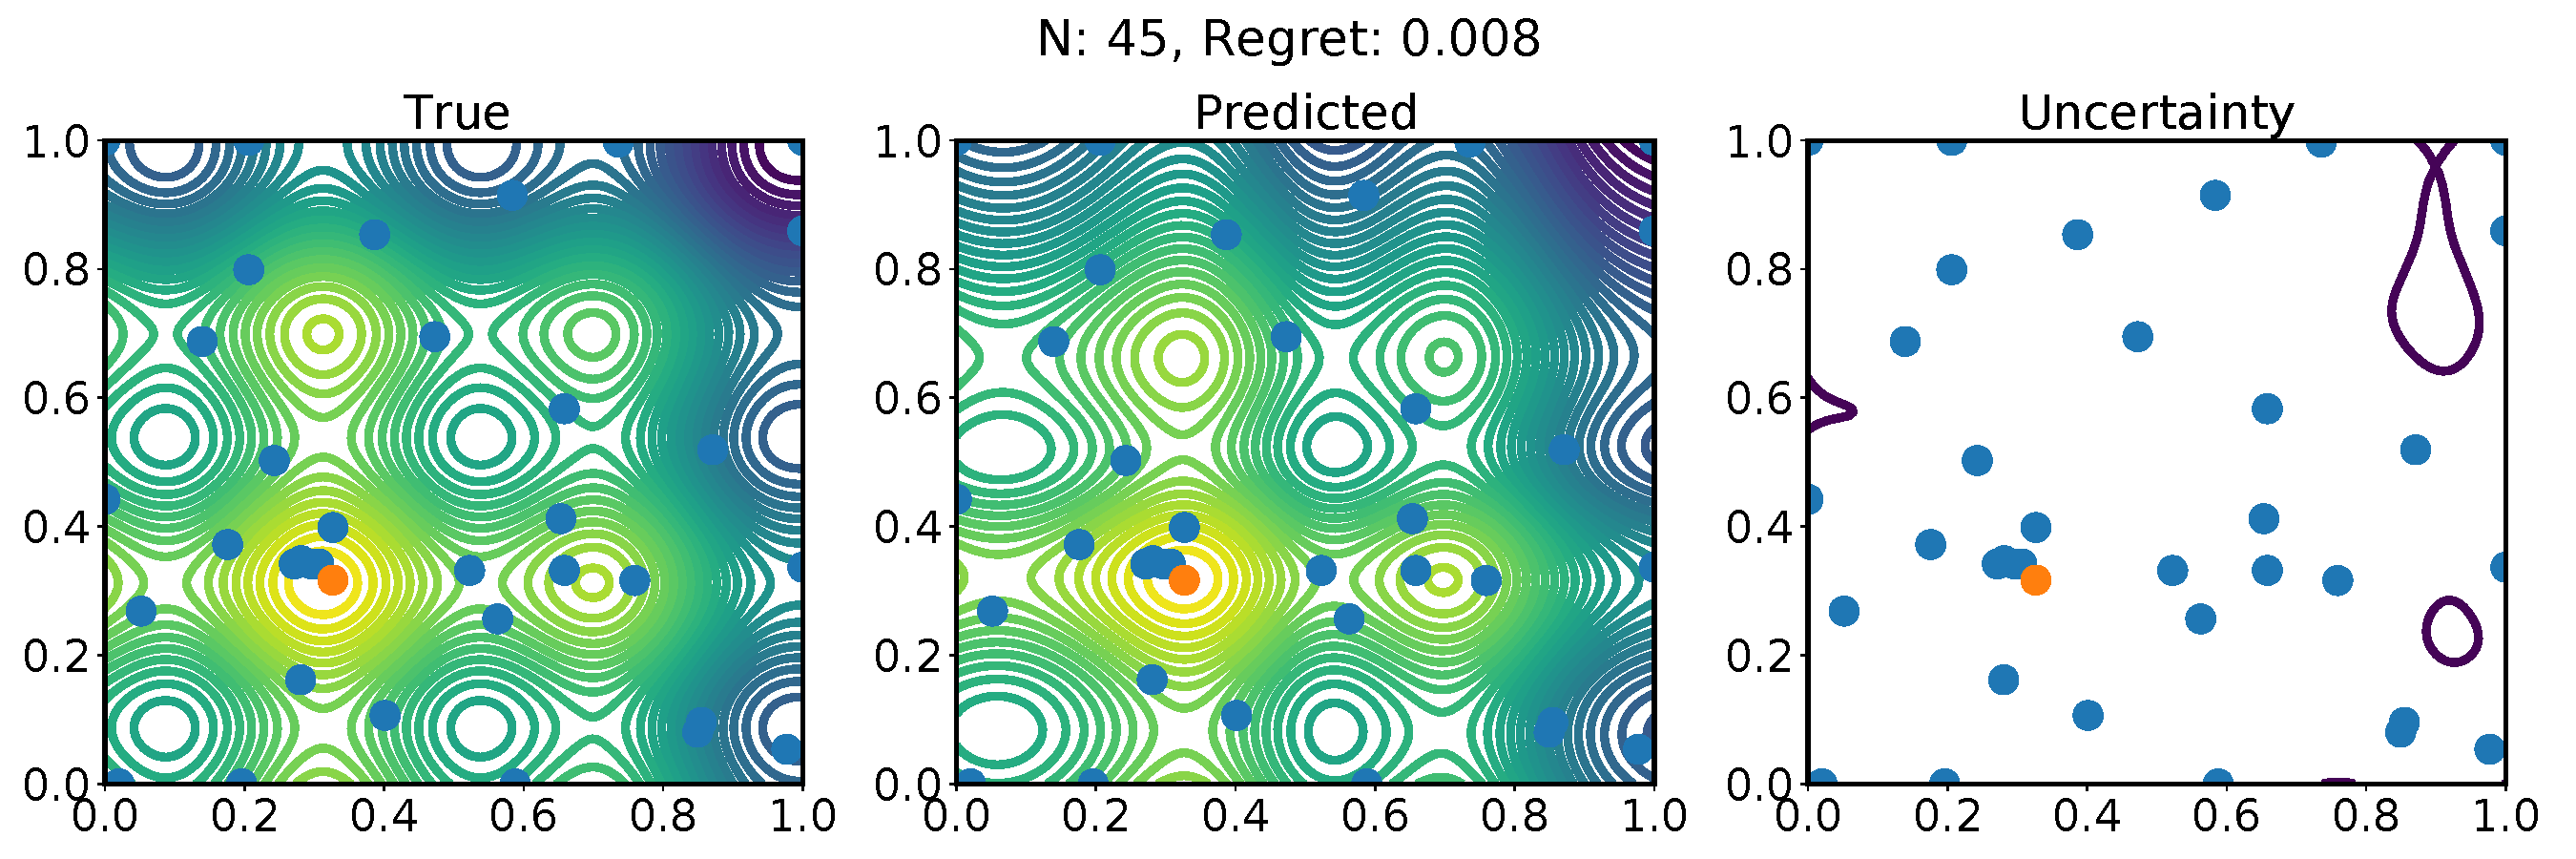
\includegraphics[width=7.5in]{Figures/Cosines_DTL_2.pdf}
\end{figure} 
~\newline

\clearpage
\section*{Method}

\subsection*{Prediction uncertainty for nonlinear parametric models}

Given variables, $\mathbf{x}$, we wish to predict the distribution of an outcome $y$ conditioned on previous observations, $\mathcal{D} = \{\mathbf{x}_i, y_i\}$. In other words, we want $p(y | \mathbf{x}, \mathcal{D})$. Using a model that depends on parameters $\theta$, the density function can be expanded and rewritten as 

\begin{equation}
p(y | \mathbf{x}, \mathcal{D}) 
= \int_{\theta} p(y, \theta | \mathbf{x}, \mathcal{D}) \mathrm{d} \theta 
= \int_{\theta} p(y | \mathbf{x}, \theta) p(\theta | \mathcal{D}) \mathrm{d} \theta.
\label{posterior predictive 1}
\end{equation}
The assumption that outcomes can be predicted by a model $f(\mathbf{x}, \theta)$ provides an expression for the data independent density of $y$, 

\begin{equation}
y = f(\mathbf{x}, \theta) + \varepsilon, \qquad \varepsilon \sim \mathcal{N}(0, \sigma^2)
\end{equation}

\begin{equation}
p(y | \mathbf{x}, \theta) = \mathcal{N} (y | f(\mathbf{x}, \theta), \sigma^2)
\label{model}
\end{equation}
where $\varepsilon$ is a random variable that models measurement noise and $\sigma^2$ is a model hyper-parameter. Bayes' theorem is used to estimate the density of model parameters given data, 

\begin{equation}
p(\theta | \mathcal{D}) = \frac{p(\mathcal{D} | \theta) p(\theta)}{p(\mathcal{D})}
\end{equation}
where the likelihood, $p(\mathcal{D} | \theta)$, is defined using equation \ref{model},

\begin{equation}
p(\mathcal{D} | \theta) = \prod_i \mathcal{N}(y_i | f(\mathbf{x}_i), \sigma^2).
\end{equation}
and the prior, $p(\theta)$, is assumed to be an isotropic Gaussian

\begin{equation}
p(\theta) = \mathcal{N}(\mathbf{0}, \alpha^{-1} \mathbb{I})
\end{equation}
where $\alpha$ is also a hyper-parameter. The Laplace approximation uses a second order Taylor series expansion to approximate the unknown density $p(\theta | \mathcal{D})$. This approximation results in a Gaussian centered at a mode of $p(\theta | \mathcal{D})$ and with a covariance matrix equal to the inverse of the matrix of second derivatives of the negative log of $p(\theta | \mathcal{D})$, 

\begin{equation}
p(\theta | \mathcal{D}) \approx \mathcal{N}(\theta | \hat{\theta}, \mathbf{H}^{-1})
\label{Laplace approximation}
\end{equation}
where

\begin{equation}
\hat{\theta} = \underset{\theta}{\text{argmax}} \; \mathrm{ln} \; p(\theta | \mathcal{D})
\end{equation}
and 
\begin{equation}
\mathbf{H} = \nabla_{\theta} \nabla_{\theta} \; -\mathrm{ln} \; \left. p(\theta | \mathcal{D}) \right|_{\theta = \hat{\theta}}.
\label{Hessian 1}
\end{equation}
Once values for $\hat{\theta}$ and $\mathbf{H}$ are obtained, model predictions are evaluated using equations \ref{posterior predictive 1}, \ref{model}, and \ref{Laplace approximation}:

\begin{equation}
p(y | \mathbf{x}, \mathcal{D}) 
= \int_{\theta} p(y | \mathbf{x}, \theta) p(\theta | \mathcal{D}) \mathrm{d} \theta 
\approx \int_{\theta} \mathcal{N} (y | f(\mathbf{x}, \theta), \sigma^2)  \mathcal{N}(\theta | \hat{\theta}, \mathbf{H}^{-1}) \mathrm{d} \theta 
\label{posterior predictive 2}
\end{equation}
Linearizing $f(\mathbf{x}, \theta)$ about $\hat{\theta}$ allows for the following approximations of the expected value and variance of $y$ given $\mathbf{x}$, where expectations are taken with respect to the parameter posterior

\begin{equation}
p(y | \mathbf{x}, \mathcal{D}) \approx \mathcal{N}(y | f(\mathbf{x}, \hat{\theta}), \sigma^2(\mathbf{x}, \hat{\theta}))
\end{equation}
where
 
\begin{equation}
\sigma^2(\mathbf{x}, \hat{\theta}) \approx \sigma^2 + \mathbf{g}(\mathbf{x}, \hat{\theta})^T \mathbf{H}^{-1} \mathbf{g}(\mathbf{x}, \hat{\theta}),
\qquad
\mathbf{g}(\mathbf{x}, \hat{\theta}) = \nabla_{\theta} \left. f(\mathbf{x}, \theta) \right|_{\theta = \hat{\theta}}
\label{variance}
\end{equation}

\clearpage
\subsection*{Approximation of Hessian inverse}
The proposed batch Bayesian optimization algorithm is based on the following approximation of the Hessian and specifically its inverse. Evaluating equation \ref{Hessian 1} gives 

\begin{align}
\mathbf{H} &= \alpha \mathbb{I} + \nabla_{\theta} \nabla_{\theta} \sum_i \sigma^{-2} (y_i - f(\mathbf{x}_i, \theta))^2  \nonumber \\
&\approx \alpha \mathbb{I} + \sigma^{-2} \sum_i \mathbf{g}(\mathbf{x}_i, \theta) \mathbf{g}(\mathbf{x}_i, \theta)^T
\end{align}
which is the outer-product approximation of the Hessian. To evaluate the inverse of the outer-product approximated Hessian, the Woodbury identity can be used to give 

\begin{equation}
\mathbf{H}_{l+1}^{-1} = \mathbf{H}_{l}^{-1} - \frac{\mathbf{H}_{l}^{-1} \mathbf{g}(\mathbf{x}_{l+1}, \theta) \mathbf{g}^T(\mathbf{x}_{l+1}, \theta) \mathbf{H}_{l}^{-1}} {\sigma^2 + \mathbf{g}^T(\mathbf{x}_{l+1}, \theta) \mathbf{H}_{l}^{-1} \mathbf{g}(\mathbf{x}_{l+1}, \theta)} 
\label{covariance update}
\end{equation}
which is evaluated sequentially with $\mathbf{H}_{0}^{-1} = 1/\alpha \mathbf{I}$. Useful features of this equation are that it provides a way to compute the inverse Hessian using a single pass through the training data and that it provides a way to update the inverse Hessian for any input, $\mathbf{x}_{l+1}$, without requiring $y_{l + 1}$!

\subsection*{Bayesian optimization and maximum expected improvement}

A common acquisition function for Bayesian optimization of $y$ with respect to $\mathbf{x}$ is the Expeceted Improvement from the best previously observed value, $y^*$, defined as 

\begin{align}
a(x) &= \mathbb{E}_{y} [ \text{max}(0, y- y^*) ]   \nonumber \\ 
&= \int_{y^*}^{\infty} (y - y^*) \mathcal{N}(y | f(\mathbf{x}, \hat{\theta}), \sigma^2(\mathbf{x})) \mathrm{d} y \nonumber \\
&= (f(\mathbf{x}, \hat{\theta}) - y^*) \Phi(f(\mathbf{x}, \hat{\theta}) | y^*, \sigma^2(\mathbf{x})) + \sigma(\mathbf{x}) \mathcal{N}(f(\mathbf{x}, \hat{\theta}) | y^*, \sigma^2(\mathbf{x})).
\label{EI}
\end{align}

\subsection*{Batch Bayesian optimization algorithm}

The proposed batch Bayesian optimization algorithm iterates between maximizing the Expected Improvement (equation \ref{EI}) acquisition function to seek an experimental condition $\mathbf{x}_{l+1}$, followed by updating the parameter covariance using equation \ref{covariance update} with $\mathbf{x}_{l+1}$. Updating the parameter covariance, $\mathbf{H}^{-1}$, affects the computation of the variance, given by equation \ref{variance}. As a result, maximizing the Expected Improvement after conditioning on $\mathbf{x}_{l+1}$ will result in a new $\mathbf{x}_{l+2}$.

%\begin{algorithm}
%\caption{Closed-loop Bayesian experimental design}
%\begin{algorithmic}
%\REQUIRE $\mathcal{D}(\mathbf{q}^{(l)})$, $f_P$, $l_{\mathrm{max}}$
%\WHILE{$l < l_{\mathrm{max}}$}
%\STATE \COMMENT{Estimate model parameter mean and covariance}
%\STATE $\theta_{\mathrm{MAP}}(\mathbf{q}^{(l)}) \leftarrow \mathop{\textrm{argmax}}_{\theta} \left[ -\mathrm{ln} \; p(\mathbf{\theta} | \mathcal{D}(\mathbf{q}^{(l)})) \right]$
%\STATE $ \mathbf{H}(\theta_{\mathrm{MAP}}(\mathbf{q}^{(l)}),\mathbf{q}^{(l)}) \leftarrow \mathbf{\Sigma}_{\theta}^{-1} + \sum_{i=1}^{n} \mathbf{G}(\theta_{\mathrm{MAP}}(\mathbf{q}^{(l)}),\mathbf{q}_i^{(l)})^T \mathbf{\Sigma}_y^{-1} \mathbf{G}(\theta_{\mathrm{MAP}}(\mathbf{q}^{(l)}),\mathbf{q}_i^{(l)})$
%\STATE \COMMENT{Design next experiment}
%\STATE $ \mathbf{q}^{(l+1)} \leftarrow \mathop{\textrm{argmax}}_{\mathbf{q}^{(l+1)} \subset \mathcal{Q} }\; \left[ f_P(\mathbf{q}^{(l+1)})
%+
%\mathrm{log} \; \mathrm{det} \;  \text{FIMB}(\theta_{\mathrm{MAP}}(\mathbf{q}^{(l)}), \mathbf{q}^{(l+1)}) \right]
%$
%\STATE \COMMENT{Collect new data, append to existing data}
%\STATE $\mathcal{D}(\mathbf{q}^{(l)}) \leftarrow \{ \mathcal{D}(\mathbf{q}^{(l)}), \mathcal{D}(\mathbf{q}^{(l+1)}) \} $ 
%\STATE $\mathbf{q}^{(l)} \leftarrow (\mathbf{q}^{(l)}, \mathbf{q}^{(l+1)})$
%\STATE $ l \leftarrow l + 1$
%\ENDWHILE
%\end{algorithmic}
%\end{algorithm}



\end{document}
